\section{Problem 2}

\subsection{Problem Statement}

\begin{figure}[H]
    \centering
    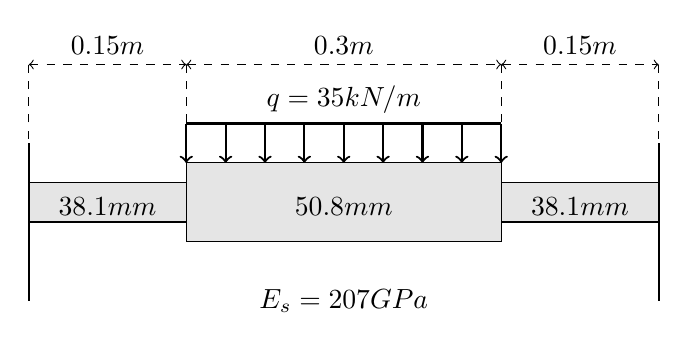
\begin{tikzpicture}
        % three part beam
        \def\beamheight{0.5}
        \def\beamwidth{2}
        \draw[fill=gray!20] (0,0) rectangle (\beamwidth,\beamheight);
        \draw[fill=gray!20] (\beamwidth, {-\beamheight/2}) rectangle ({3*\beamwidth},{1.5*\beamheight});
        \draw[fill=gray!20] ({3*\beamwidth}, 0) rectangle ({4*\beamwidth},{\beamheight});
        % insert to walls on both sides
        \draw[thick] (0, -1) -- (0, 1);
        \draw[thick] ({4*\beamwidth}, -1) -- ({4*\beamwidth}, 1);
        % 0.15m for 2 side parts
        % 0.3m for middle part
        \draw[dashed] (0, 0) -- (0, {4*\beamheight});
        \draw[dashed] (\beamwidth, 0) -- (\beamwidth, {4*\beamheight});
        \draw[<->, dashed] (0, {4*\beamheight}) -- (\beamwidth, {4*\beamheight}) node[midway, above] {$0.15m$};

        \draw[dashed] ({3*\beamwidth}, 0) -- ({3*\beamwidth}, {4*\beamheight});
        \draw[dashed] ({4*\beamwidth}, 0) -- ({4*\beamwidth}, {4*\beamheight});
        \draw[<->, dashed] ({3*\beamwidth}, {4*\beamheight}) -- ({4*\beamwidth}, {4*\beamheight}) node[midway, above] {$0.15m$};

        \draw[dashed] (\beamwidth, 0) -- (\beamwidth, {4*\beamheight});
        \draw[dashed] ({3*\beamwidth}, 0) -- ({3*\beamwidth}, {4*\beamheight});
        \draw[<->, dashed] (\beamwidth, {4*\beamheight}) -- ({3*\beamwidth}, {4*\beamheight}) node[midway, above] {$0.3m$};

        \draw[thick] (\beamwidth, {2.5*\beamheight}) -- ({3*\beamwidth}, {2.5*\beamheight}) node[midway, above] {$q=35kN/m$};
        % distributed force in center beam
        \foreach \x in {0, 0.5, ..., 4}
            \draw[->, thick] ({\beamwidth+\x}, {2.5*\beamheight}) -- ({\beamwidth+\x}, {1.5*\beamheight});

        % diameter
        \node at ({\beamwidth/2}, 0.2) {$38.1mm$};
        \node at ({3*\beamwidth+\beamwidth/2}, 0.2) {$38.1mm$};
        \node at ({2*\beamwidth}, 0.2) {$50.8mm$};
        \node at ({2*\beamwidth}, -1) {$E_s=207GPa$};
    \end{tikzpicture}
    \caption{Problem 2}
    \label{fig:problem2}
\end{figure}

As seen in Figure \ref{fig:problem2}, the beam is made of three parts, with the left and right parts having the same length of $0.15m$, and the middle part having the length of $0.3m$. The diameter of the left and right parts is $38.1mm$, and the diameter of the middle part is $50.8mm$. The beam is made of steel with the Young's modulus of $207GPa$. The beam is subjected to a distributed force of $35kN/m$ in the middle part.

We will first propose an analytical solution to this problem, and then use finite element method to solve this problem. 
The results will be compared between FEM code and analytical solution.

\subsection{Analytical Solution}

\subsubsection{Symmetrical Analysis}

For the symmetrical problem, 
we can divide the beam into two parts at the middle.
\begin{figure}[H]
    \centering
    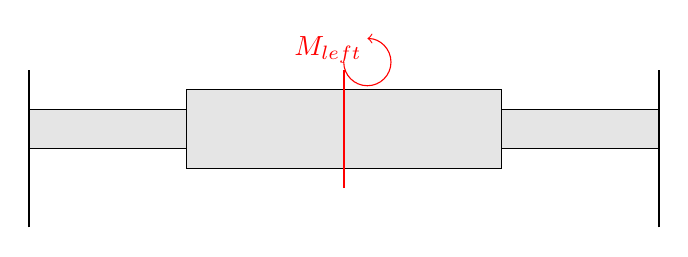
\begin{tikzpicture}
        % three part beam
        \def\beamheight{0.5}
        \def\beamwidth{2}
        \draw[fill=gray!20] (0,0) rectangle (\beamwidth,\beamheight);
        \draw[fill=gray!20] (\beamwidth, {-\beamheight/2}) rectangle ({3*\beamwidth},{1.5*\beamheight});
        \draw[fill=gray!20] ({3*\beamwidth}, 0) rectangle ({4*\beamwidth},{\beamheight});
        % insert to walls on both sides
        \draw[thick] (0, -1) -- (0, 1);
        \draw[thick] ({4*\beamwidth}, -1) -- ({4*\beamwidth}, 1);
        
        \draw[thick, red] ({2*\beamwidth}, {-\beamheight}) -- ({2*\beamwidth}, {2*\beamheight});

        % draw a torque in the middle
        \draw[->, red] ({2*\beamwidth}, {2.2*\beamheight}) arc (-180:90:0.3);
        \node[red] at ({1.9*\beamwidth}, {2.5*\beamheight}) {$M_{\text{left}}$};
    \end{tikzpicture}
    \caption{Symmetrical Problem}
\end{figure}

In Material Mechanics, for a symmetrical problem, 
internal force and moment in the middle part excludes torsion $F_s$ but 
includes bending moment $M_s$ and axial force $F_N$.
For the left beam system part, 
the effect of right beam system part can be reduced to 
a simple bending moment $M_{\text{left}}$.

What's more, the rotation angle $\theta$ in the middle 
is $0$ for such symmetrical problem.

With superposition principle, 
the rotation angle $\theta$ at the middle is contributed by $q$ and 
$M_{L} = M_{\text{left}}$.Denote:
\begin{itemize}
    \item $L=0.15m$;
    \item $E=E_s=207GPa$;
    \item $q=35kN/m$;
    \item $J_1=\frac{\pi}{64}d_1^4$, $J_2=\frac{\pi}{64}d_2^4$;
    \item $M_L = M_{\text{left}}$;
\end{itemize}

$\theta$ in the middle part can be devided into two parts:
\begin{equation}
    \theta = \theta_M + \theta_q
\end{equation}
where $\theta_M$ is the rotation angle caused by $M_L$, and $\theta_q$ is the rotation angle caused by $q$.
$\theta_M$ can be calculated by:
\begin{equation}
    \theta_M = \frac{L M_{L}}{E J_{2}} + \frac{L M_{L}}{E J_{1}}
\end{equation}

$\theta_q$ can be calculated by $2$ parts.
One part $\theta_q^1$ is contributed by left beam part, 
and the other part $\theta_q^2$ is contributed by middle beam part.
\begin{equation}
    \theta_q = \theta_q^1 + \theta_q^2
\end{equation}

$\theta_q^1$ can be calculated by the equivalent force system of $q$ applied on the left beam part (seen in 
Figure \ref{fig:problem2_equivalent_force_system}):
\begin{equation}
    \theta_q^1 = -\frac{q L L^2}{2 E J_{1}}
    - \frac{\frac{1}{2}qL^2 L}{E J_{1}}=
    - \frac{L^{3} q}{E J_{1}}
\end{equation}

\begin{figure}[H]
    \centering
    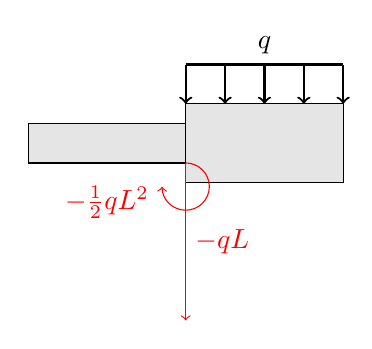
\begin{tikzpicture}
        \def\beamheight{0.5}
        \def\beamwidth{2}
        \draw[fill=gray!20] (0,0) rectangle (\beamwidth,\beamheight);
        \draw[fill=gray!20] (\beamwidth, {-\beamheight/2}) rectangle ({2*\beamwidth},{1.5*\beamheight});
        % q
        \foreach \x in {0, 0.5, ..., 2}
            \draw[->, thick] ({\beamwidth+\x}, {2.5*\beamheight}) -- ({\beamwidth+\x}, {1.5*\beamheight});
        \draw[thick] (\beamwidth, {2.5*\beamheight}) -- ({2*\beamwidth}, {2.5*\beamheight}) node[midway, above] {$q$};
        % force
        \draw[->, red] ({\beamwidth}, 0) -- ({\beamwidth}, -2) node[midway, right] {$-qL$};
        % moment arc
        \draw[->, red] ({\beamwidth}, 0) arc (90:-180:0.3);
        \node[red] at ({\beamwidth/2}, -0.5) {$-\frac{1}{2}qL^2$};
    \end{tikzpicture}
    \caption{Equivalent Force System of $q$ on Left Beam Part}
    \label{fig:problem2_equivalent_force_system}
\end{figure}
$\theta_q^2$ is contributed by $q$ on the middle beam part:
\begin{equation}
    \theta_q^2 = -\frac{qL^3}{6EJ_2}
\end{equation}
thus $\theta_q$ is:
\begin{equation}
    \theta_q = - \frac{L^{3} q}{6 E J_{2}} - \frac{L^{3} q}{E J_{1}}
\end{equation}
for $\theta_q + \theta_M = 0$, we have:
\begin{equation}
    - \frac{L^{3} q}{6 E J_{2}} + \frac{L M_{L}}{E J_{2}} - \frac{L^{3} q}{E J_{1}} + \frac{L M_{L}}{E J_{1}} = 0
\end{equation}
finally, we have $M_L$:
\begin{equation}
    M_{L} = \frac{L^{2} q \left(J_{1} + 6 J_{2}\right)}{6 \left(J_{1} + J_{2}\right)}
\end{equation}

\subsubsection{Distribution of $\theta$}

$\theta(x)$ can also calculated by $2$ parts:
\begin{equation}
    \theta(x) = \theta_M(x) + \theta_q(x)
\end{equation}

For $0 \leq x \leq L$, $\theta_M(x)$ is:
\begin{equation}
    \theta_M(x) = 
    \frac{M_L x}{EJ_1}=
    \frac{L^{2} q x \left(J_{1} + 6 J_{2}\right)}{6 E J_{1} \left(J_{1} + J_{2}\right)}
\end{equation}
and $\theta_q(x)$ is:
\begin{equation}
    \theta_q(x)=
    -\frac{qL x^2}{EJ_1}-
    \frac{qL\left(L-x+\frac{L}{2}\right)}{EJ_1}=
    \frac{L q x \left(- 3 L + x\right)}{2 E J_{1}}
\end{equation}
thus $\theta(L)$ is:
\begin{equation}
    \theta(L) = 
    - \frac{L^{3} q}{E J_{1}} + \frac{L^{3} q \left(J_{1} + 6 J_{2}\right)}{6 E J_{1} \left(J_{1} + J_{2}\right)}
\end{equation}

And for $L \leq x \leq 2L$, $\theta(x)=\theta_M(x) + \theta_q(x) + \theta(L)$, where
$\theta_M(x)$ is:
\begin{equation}
    \theta_M(x) = 
    \frac{M_L (x-L)}{EJ_2}=
    \frac{L^{2} q (x-L) \left(J_{1} + 6 J_{2}\right)}{6 E J_{2} \left(J_{1} + J_{2}\right)}
\end{equation}
and for $\theta_q(x)$, we have:
\begin{equation}
    \begin{aligned}
        \theta_q(x) &= 
    -\frac{q(x-L)^3}{6EJ_2}-
    \frac{q(2L-x) (x-L)^2}{2EJ_2}-
    \frac{\frac{1}{2}q (2L-x)^2 (x-L)}{EJ_2}\\
    &=
    \frac{q \left(7 L^{3} - 12 L^{2} x + 6 L x^{2} - x^{3}\right)}{6 E J_{2}}
    \end{aligned}
\end{equation}
finally we have $\theta(x)$ at $L \leq x \leq 2L$:
\begin{equation}
    \begin{aligned}
        \theta(x)&=
        \theta_M(x) + \theta_q(x) + \theta(L)\\
        &=
        \frac{q \left(6 J_{1} L^{3} - 11 J_{1} L^{2} x + 6 J_{1} L x^{2} - J_{1} x^{3} - 4 J_{2} L^{3} - 6 J_{2} L^{2} x + 6 J_{2} L x^{2} - J_{2} x^{3}\right)}{6 E J_{2} \left(J_{1} + J_{2}\right)}
    \end{aligned}
\end{equation}
thus we have the distribution of $\theta(x)$:
\begin{equation}
    \theta(x)=
    \begin{cases}
        \frac{L^{2} q x \left(J_{1} + 6 J_{2}\right)}{6 E J_{1} \left(J_{1} + J_{2}\right)} + \frac{L q x \left(- 3 L + x\right)}{2 E J_{1}}\quad &0 \leq x \leq L\\
        \frac{q \left(6 J_{1} L^{3} - 11 J_{1} L^{2} x + 6 J_{1} L x^{2} - J_{1} x^{3} - 4 J_{2} L^{3} - 6 J_{2} L^{2} x + 6 J_{2} L x^{2} - J_{2} x^{3}\right)}{6 E J_{2} \left(J_{1} + J_{2}\right)}
        \quad &L \leq x \leq 2L
    \end{cases}
\end{equation}
the other half of the beam can be calculated by symmetry.

\subsubsection{Distribution of $w(x)$}

Similar to the derivation of $\theta(x)$,
$w(x)$ can be calculated by $2$ parts:
\begin{equation}
    w(x) = w_M(x) + w_q(x)
\end{equation}

For $0 \leq x \leq L$, $w_M(x)$ is:
\begin{equation}
    w_M(x) =
    \frac{M_L x^2}{2EJ_1}=
    \frac{L^{2} q x^{2} \left(J_{1} + 6 J_{2}\right)}{12 E J_{1} \left(J_{1} + J_{2}\right)}
\end{equation}
and $w_q(x)$ is:
\begin{equation}
    w_q(x) =
    -\frac{qL x^3}{3EJ_1}-
    \frac{qL\left(L-x+\frac{L}{2}\right)x^2}{2EJ_1}=
    \frac{L q x^{2} \left(- 9 L + 2 x\right)}{12 E J_{1}}
\end{equation}
thus for $0 \leq x \leq L$, $w(x)$ is:
\begin{equation}
    w(x) = 
    \frac{L q x^{2} \left(L \left(J_{1} + 6 J_{2}\right) - \left(J_{1} + J_{2}\right) \left(9 L - 2 x\right)\right)}{12 E J_{1} \left(J_{1} + J_{2}\right)}
\end{equation}
which is exactly the integral of $\theta(x)$.
And for $x=L$:
\begin{equation}
    w(L) = - \frac{L^{4} q \left(6 J_{1} + J_{2}\right)}{12 E J_{1} \left(J_{1} + J_{2}\right)}
\end{equation}

For $L \leq x \leq 2L$, $w_M(x)$ is:
\begin{equation}
    w_M(x) =
    \frac{M_L (x-L)^2}{2EJ_2}=
    \frac{L^{2} q \left(J_{1} + 6 J_{2}\right) \left(L - x\right)^{2}}{12 E J_{2} \left(J_{1} + J_{2}\right)}
\end{equation}
and $w_q(x)$ is:
\begin{equation}
    \begin{aligned}
        w_q(x) &=
            -\frac{q(x-L)^4}{8EJ_2}-
            \frac{q(2L-x) (x-L)^3}{3EJ_2}-
            \frac{\frac{1}{2}q (2L-x)^2 (x-L)^2}{2EJ_2}\\
        &=
        \frac{J_{1} L^{4} q}{12 E J_{1} J_{2} + 12 E J_{2}^{2}} - \frac{6 J_{1} L^{4} q}{12 E J_{1}^{2} + 12 E J_{1} J_{2}} \\
        &- \frac{J_{1} L^{4} q}{6 E J_{1}^{2} + 6 E J_{1} J_{2}} - \frac{2 J_{1} L^{3} q x}{12 E J_{1} J_{2} + 12 E J_{2}^{2}} \\
        &+ \frac{J_{1} L^{3} q x}{6 E J_{1}^{2} + 6 E J_{1} J_{2}} + \frac{J_{1} L^{2} q x^{2}}{12 E J_{1} J_{2} + 12 E J_{2}^{2}} \\
        &+ \frac{6 J_{2} L^{4} q}{12 E J_{1} J_{2} + 12 E J_{2}^{2}} - \frac{J_{2} L^{4} q}{12 E J_{1}^{2} + 12 E J_{1} J_{2}} \\
        &- \frac{6 J_{2} L^{4} q}{6 E J_{1}^{2} + 6 E J_{1} J_{2}} - \frac{12 J_{2} L^{3} q x}{12 E J_{1} J_{2} + 12 E J_{2}^{2}} \\
        &+ \frac{6 J_{2} L^{3} q x}{6 E J_{1}^{2} + 6 E J_{1} J_{2}} + \frac{6 J_{2} L^{2} q x^{2}}{12 E J_{1} J_{2} + 12 E J_{2}^{2}} \\
        &- \frac{11 L^{4} q}{24 E J_{2}} + \frac{7 L^{3} q x}{6 E J_{2}} - \frac{L^{2} q x^{2}}{E J_{2}} + \frac{L q x^{3}}{3 E J_{2}} - \frac{q x^{4}}{24 E J_{2}} + \frac{L^{4} q}{E J_{1}} - \frac{L^{3} q x}{E J_{1}}
    \end{aligned}
\end{equation}
thus for $L \leq x \leq 2L$, $w(x)$ is:
\begin{equation}
    w(x)=
    w_q(x) + w_M(x) + w(L) + \theta(L)(x-L)
\end{equation}
which is exactly the integral of $\theta(x)$.
Finally we have the distribution of $w(x)$ (too long to write here).

\subsubsection{Figure of $\theta(x)$ and $w(x)$'s Distribution}

Substitute the numerical values into the equations above,
we have the distribution of $\theta(x)$ and $w(x)$.

\begin{figure}[H]
    \centering
    \includegraphics[width=0.7\linewidth]{../problem2/images/deflection_angle_analytical.pdf}
    \caption{$\theta(x)$'s Distribution}
\end{figure}

\begin{figure}[H]
    \centering
    \includegraphics[width=0.7\linewidth]{../problem2/images/deflection_analytical.pdf}
    \caption{$w(x)$'s Distribution}
\end{figure}
The detailed derivation can be found in 
\verb|problem2/src/analytical.py| or 
\verb|problem2/draft/analytical.ipynb|, 
which uses \verb|sympy| to do the symbolic calculation.
I shall not present the derivation code here.

\subsection{Julia Code Solution}

You may find the detailed derivation in last year's report or my video.
To conclude, 
we have the relation on this cell part as the format $[K]u=b$:
\begin{equation}
    EJ
    \begin{bmatrix}
        \frac{12}{h^3} & \frac{6}{h^2} & -\frac{12}{h^3} & \frac{6}{h^2} \\
        \frac{6}{h^2} & \frac{4}{h} & -\frac{6}{h^2} & \frac{2}{h} \\
        -\frac{12}{h^3} & -\frac{6}{h^2} & \frac{12}{h^3} & -\frac{6}{h^2} \\
        \frac{6}{h^2} & \frac{2}{h} & -\frac{6}{h^2} & \frac{4}{h} \\
       \end{bmatrix}
       \begin{bmatrix}
           w_1\\ \theta_1\\ w_2\\ \theta_2
       \end{bmatrix}
       =
       q_{ex}
       \begin{bmatrix}
        \frac{h}{2}\\
        \frac{h^2}{12}\\
        \frac{h}{2}\\
        -\frac{h^2}{12}
        \end{bmatrix}
        +
        \begin{bmatrix}
            0\\
            0\\
            F_{ex}\\
            -M_{ex}
        \end{bmatrix}
\end{equation}

And the application of $q_{ex}, F_{ex}, M_{ex}$ is shown in fig.\ref{Bernoulli-Euler beam element}.

\begin{figure}[H]
    \centering
    \begin{tikzpicture}
        \draw[-](0, 0)--(5, 0);
        \draw[-](0, 0)--(0, 0.3);
        \draw[-](5, 0)--(5, 0.3);
        \node at (0, -0.3) {$x_1$};
        \node at (5, -0.3) {$x_2$};
        \node at (2.5, -0.5) {$h$};

        \draw[->] (5, -3)--(5, -2);
        \node at (5, -3.3) {$F_{ex}$};

        \node at (0, 0.6) {$w_1$};
        \node at (0, 1.2) {$\theta_1$};
        \node at (5, 0.6) {$w_2$};
        \node at (5, 1.2) {$\theta_2$};

        \draw[<->] (5.1, -1)--(5.5, -1)--(5.5, 1)--(5.9, 1);
        \node at (5.9, 0) {$M_{ex}$};

        \draw[-] (0, -1.5)--(5, -1.5);
        \foreach \i in {0,0.5,1,...,5}{
            \draw[->] (\i, -1.5) -- (\i, -1);
        };
        \node at (2.5, -2) {$q_{ex}$};
    \end{tikzpicture}
    \caption{Bernoulli-Euler beam element}
    \label{Bernoulli-Euler beam element}
\end{figure}

What's more, 
after calculation, 
minor-interpolation is used to get the value distributed 
inside an element (cell).
This part can also be seen in last year's report.

For this year's task requires to use the 
minimum element number to achieve the accuracy,
I make a comparison between $2$ cases:
\begin{itemize}
    \item $3$ elements, with one elements in two sides and one element in the middle;
    \item $4$ elements, an extra element is added in the middle.
\end{itemize}

At the beginning, 
I think $3$ elements is enough to achieve the accuracy.
However,
I find that the error is still large.
Thus I add an extra element in the middle,
whose results quite fits for the analytical solution.
The julia code is shown below.

First, 
import the necessary packages,
where \verb|LinearAlgebra| is used to do matrix calculation,
\verb|CairoMakie| is used to plot the figure,
and \verb|SparseArrays| is used to store the sparse matrix.
\begin{lstlisting}[language=matlab]
using LinearAlgebra, CairoMakie, SparseArrays;
\end{lstlisting}

Then, we define a struct of \verb|HermiteBeam| and
its constructor:
\begin{lstlisting}[language=matlab]
struct HermiteBeam
    n_nodes_::Int
    n_elements_::Int
    x_mesh_::Vector{Float64}
    h_::Float64
    e_s_::Float64
    inertia_::Float64
    q_::Float64
end

function HermiteBeam(n_nodes::Int, x_0::Float64, beam_length::Float64, e_s::Float64, inertia::Float64, q::Float64)
    h = beam_length / (n_nodes - 1);
    x_mesh = Vector(LinRange(x_0, x_0 + beam_length, n_nodes));
    return HermiteBeam(n_nodes, n_nodes-1, x_mesh, h, e_s, inertia, q);
end
\end{lstlisting}

By the derivation above and in last year's report,
the stiffness matrix $[K]$ and force vector $b$ can be calculated as below:
\begin{lstlisting}[language=matlab]
function generateBeamFEM(hermite_beams::Vector{HermiteBeam})
    n_nodes = sum([hermite_beam.n_nodes_ for hermite_beam in hermite_beams]);
    n_nodes -= length(hermite_beams) - 1;
    stiffness_matrix = spzeros(2*n_nodes, 2*n_nodes);
    source_vector = zeros(2*n_nodes);
    for (i_beam, beam) in enumerate(hermite_beams)
        start_node_id = sum([b.n_nodes_ for b in hermite_beams[1:i_beam-1]]) - (i_beam - 1);
        h = beam.h_;
        part_stiffness_matrix = [
            12/h^3 6/h^2 -12/h^3 6/h^2;
            6/h^2 4/h -6/h^2 2/h;
            -12/h^3 -6/h^2 12/h^3 -6/h^2;
            6/h^2 2/h -6/h^2 4/h
        ] * beam.e_s_ * beam.inertia_;
        part_source_vector = [h/2, h^2/12, h/2, -h^2/12] * beam.q_;
        # insert part stiffness matrix to stiffness matrix
        # and part source vector to source vector
        for i_element = 1: beam.n_elements_
            stiffness_matrix[
                2*start_node_id + 2*i_element - 1: 2*start_node_id + 2*i_element + 2,
                2*start_node_id + 2*i_element - 1: 2*start_node_id + 2*i_element + 2
            ] .+= part_stiffness_matrix;
            source_vector[
                2*start_node_id + 2*i_element - 1: 2*start_node_id + 2*i_element + 2
            ] .+= part_source_vector;
        end
    end
    return stiffness_matrix, source_vector;
end
\end{lstlisting}

For we need compare $2$ cases,
we define a struct of \verb|Problem| as below,
as well as a function to generate the \verb|HermiteBeam|s:
\begin{lstlisting}[language=matlab]
struct Problem
    e_s_::Vector{Float64}
    j_::Vector{Float64}
    l_::Vector{Float64}
    n_::Vector{Int}
    q_::Vector{Float64}
end

function generateHermiteBeams(problem::Problem)
    hermite_beams = HermiteBeam[];
    for i = 1: length(problem.e_s_)
        n = problem.n_[i];
        beam_length = problem.l_[i];
        start_x = sum(problem.l_[1:i]) - beam_length;
        e_s = problem.e_s_[i];
        inertia = problem.j_[i];
        q = problem.q_[i];
        hermite_beam = HermiteBeam(n, start_x, beam_length, e_s, inertia, q);
        push!(hermite_beams, hermite_beam);
    end
    return hermite_beams;
end
\end{lstlisting}

For the beam is hanged on both sides towards the wall,
the Dirichlet boundary condition is $0$ for $w$ and $\theta$ 
at the beginning and the end of the beam:
\begin{lstlisting}[language=matlab]
function knownNodes(problem::Problem)
    known_nodes_ids = [1, 2, 2*(sum(problem.n_) - length(problem.n_) + 1)-1, 2*(sum(problem.n_) - length(problem.n_) + 1)];
    known_nodes_values = [0., 0., 0., 0.];
    return known_nodes_ids, known_nodes_values;
end
\end{lstlisting}

Similar to problem 1, 
the \verb|solve| function is defined as below:
\begin{lstlisting}[language=matlab]
function solve(
    stiffness_matrix::SparseMatrixCSC, 
    source_vector::Vector, 
    known_nodes_ids::Vector,
    known_nodes_values::Vector
)::Vector
    @assert length(known_nodes_ids) == length(known_nodes_values);
    n_nodes = length(source_vector);
    solution_vector = zeros(n_nodes);
    solution_vector[known_nodes_ids] .= known_nodes_values;
    unknown_nodes_ids = setdiff(1:n_nodes, known_nodes_ids);
    part_stiffness_matrix = stiffness_matrix[unknown_nodes_ids, unknown_nodes_ids];
    part_source_vector = (source_vector .- stiffness_matrix * solution_vector)[unknown_nodes_ids];
    solution_vector[unknown_nodes_ids] .= part_stiffness_matrix \ part_source_vector;
    return solution_vector;
end
\end{lstlisting}

Next, let's use the \verb|solve| function to solve the problem,
and return the solution $w$ and $\theta$ at given nodes:
\begin{lstlisting}[language=matlab]
function solveProblem(problem::Problem)
    hermite_beams = generateHermiteBeams(problem);
    stiffness_matrix, source_vector = generateBeamFEM(hermite_beams);
    known_nodes_ids, known_nodes_values = knownNodes(problem);
    solution_vector = solve(stiffness_matrix, source_vector, known_nodes_ids, known_nodes_values);
    w = solution_vector[1:2:end];
    theta = solution_vector[2:2:end];
    return hermite_beams, w, theta;
end
\end{lstlisting}

As soon as the solution is obtained,
a minor-interpolation is used to get the value distributed
inside each element (cell),
this derivation can be found in last year's report:
\begin{lstlisting}[language=matlab]
function hermiteInterpolation(
    hermite_beams::Vector{HermiteBeam},
    ws::Vector,
    thetas::Vector,
    x::Float64
)
    for (i_beam, beam) in enumerate(hermite_beams)
        if x < beam.x_mesh_[1] || x > beam.x_mesh_[end]
            continue;
        else
            start_node_id = sum([b.n_nodes_ for b in hermite_beams[1:i_beam-1]]) - (i_beam - 1);
            w_beam = ws[start_node_id+1: start_node_id+beam.n_nodes_];
            theta_beam = thetas[start_node_id+1: start_node_id+beam.n_nodes_];
            if x in beam.x_mesh_
                index = findfirst(isequal(x), beam.x_mesh_);
                return w_beam[index], theta_beam[index];
            else
                index = findfirst(item->item > x, beam.x_mesh_);
                # if index == 1
                #     index = 2;
                # end
                index -= 1;
                x1 = beam.x_mesh_[index];
                t = x - x1;
                h = beam.h_;
                w_theta = [w_beam[index], theta_beam[index], w_beam[index+1], theta_beam[index+1]];
                coeff1 = [
                    (h-t)^2 * (h + 2*t), t * (h-t)^2 * h, t^2 * (3*h - 2*t), t^2 * (t-h) * h
                ] ./ h^3;
                coeff2 = [
                    6 * t * (t-h), (h - 3*t) * (h - t) * h, 6 * t * (h-t), t * (3*t - 2*h) * h
                ] ./ h^3;
                return dot(coeff1, w_theta), dot(coeff2, w_theta);
            end
        end
    end
    return 0., 0.;
end

function hermiteInterpolation(
    hermite_beams::Vector{HermiteBeam},
    ws::Vector,
    thetas::Vector,
    x_mesh_minor::Vector
)
    theta_minor = similar(x_mesh_minor);
    w_minor = similar(x_mesh_minor);
    for (i, x) in enumerate(x_mesh_minor)
        w_minor[i], theta_minor[i] = hermiteInterpolation(hermite_beams, ws, thetas, x);
    end
    return w_minor, theta_minor;
end
\end{lstlisting}

Let's define a function to solve the problem and minor-interpolate the solution:
\begin{lstlisting}[language=matlab]
function solveAndMinor(problem::Problem, x_minor::Vector)
    hermite_beams, w, theta = solveProblem(problem);
    w_minor, theta_minor = hermiteInterpolation(hermite_beams, w, theta, x_minor);
    return w_minor, theta_minor;
end
\end{lstlisting}

Now, let's define $2$ cases of problem and solve them as follows:
\begin{lstlisting}[language=matlab]
e_s = zeros(3) .+ 207e9;
j = [38.1e-3, 50.8e-3, 38.1e-3] .^4 .* pi ./ 64;
l = [0.15, 0.3, 0.15];
n1 = [2, 2, 2];
n2 = [2, 3, 2];
q = [0., -35e3, 0.];

problem_1 = Problem(e_s, j, l, n1, q);
problem_2 = Problem(e_s, j, l, n2, q);

x_minor = Vector(LinRange(0., sum(problem_1.l_), 101));
w_minor_1, theta_minor_1 = solveAndMinor(problem_1, x_minor);
w_minor_2, theta_minor_2 = solveAndMinor(problem_2, x_minor);
\end{lstlisting}

To compare the results with analytical solution,
I print the analytical solution using \verb|sympy|,
and transform the \verb|sympy| expression to \verb|julia| expression using 
\verb|codegen| module in \verb|sympy|:
\begin{lstlisting}[language=matlab]
function analyticalAngle(x)
    out1 = ((x <= 0.15) ? (x .* (0.122599630386343 * x - 0.0257568362948163)) : (-0.0862028651153974 * x .^ 3 + 0.0775825786038577 * x .^ 2 - 0.013968317379196 * x - 0.000464459502472649))
    return out1
end

function analyticalDeflection(x)
    out1 = ((x <= 0.15) ? (x .^ 2 .* (0.0408665434621143 * x - 0.0128784181474081)) : (-0.0215507162788494 * x .^ 4 + 0.0258608595346192 * x .^ 3 - 0.00698415868959802 * x .^ 2 - 0.000464459502472649 * x - 1.39767905836677e-6))
    return out1
end

x_analytical = Vector(LinRange(0., sum(problem_1.l_)/2, 21));
w_analytical = analyticalDeflection.(x_analytical);
theta_analytical = analyticalAngle.(x_analytical);
\end{lstlisting}

Finally, let's plot the results using \verb|CairoMakie|:
\begin{lstlisting}[language=matlab]
# w figure
fig_w = Figure(resolution = (800, 600), fontsize = 20);
axes_w = Axis(fig_w[1, 1], xlabel = L"$x$", ylabel = L"$w$", title = "Deflection");
lines!(axes_w, x_minor, w_minor_1, color = :blue, linewidth = 2, label = L"$n_2=2$");
lines!(axes_w, x_minor, w_minor_2, color = :green, linewidth = 2, label = L"$n_2=3$");
scatter!(axes_w, x_analytical, w_analytical, color = :red, linewidth = 2, label = "Analytical");
axislegend(axes_w, framevisible = true, position=:rb);
save("../images/deflection.pdf", fig_w, pt_per_unit = 0.7);
save("../images/deflection.png", fig_w);
fig_w
    
# theta figure
fig_theta = Figure(resolution = (800, 600), fontsize = 20);
axes_theta = Axis(fig_theta[1, 1], xlabel = L"$x$", ylabel = L"$\theta$", title = "Angle");
lines!(axes_theta, x_minor, theta_minor_1, color = :blue, linewidth = 2, label = L"$n_2=2$");
lines!(axes_theta, x_minor, theta_minor_2, color = :green, linewidth = 2, label = L"$n_2=3$");
scatter!(axes_theta, x_analytical, theta_analytical, color = :red, linewidth = 2, label = "Analytical");
axislegend(axes_theta, framevisible = true, position=:rb);
save("../images/angle.pdf", fig_theta, pt_per_unit = 0.7);
save("../images/angle.png", fig_theta);
fig_theta
\end{lstlisting}

The result is shown in fig.\ref{fig:problem2_w} and fig.\ref{fig:problem2_theta}.

\begin{figure}[H]
    \centering
    \includegraphics[width=\linewidth]{../problem2/images/deflection.pdf}
    \caption{$w(x)$'s Distribution and Comparison}
    \label{fig:problem2_w}
\end{figure}

\begin{figure}[H]
    \centering
    \includegraphics[width=\linewidth]{../problem2/images/angle.pdf}
    \caption{$\theta(x)$'s Distribution and Comparison}
    \label{fig:problem2_theta}
\end{figure}

Although I check the solution of $n_2=2$ and
$n_2=3$ (which means number of nodes in the middle beam,
representing $1$ and $2$ elements at middle),
they share the same result of $w$ and $\theta$ 
at the connecting point of the middle beam and the side beams.
However,
for interpolation is used to get the value inside the element,
the result of $n_2=2$ and $n_2=3$ is different inside the middle element.

The figure above turns out that $n_2=3$ is more accurate than $n_2=2$, 
compared with the analytical solution.
Thus, I think the minimum element number to achieve the accuracy in 
such problem is $4$,
with $1$ element in left and right beam,
and $2$ elements in the middle beam.